\section{Egyedek tulajdonságainak összehasonlítása és reprezentálása}
A továbbiakban egy népszerű játékból kigyűjtött adatok vizualizációját fogom elvégezni és ezáltal bemutatni az eszköz képességét, és testreszabhatóságát. Az adathalmaz a Pokemonok első generációjának az adatait foglalja magába, amely nyilvánosan elérhető. Az adatok importálása egyszerűen történik. Az adat tábla tartalmát a \ref{fig:pokedata}. ábra mutatja be. Minden Pokemon rendelkezik 3 fő attribútummal, amelyek a következőek: Name, Primary(Type), Secondary(Type). A többi mező pedig egyszerű metrika, amelyek az adott egyed támadó/védekező és egyéb a játékban használt tulajdonságait reprezentálja egy egységes rendszerben. 

\begin{figure}[h!]
	\centering
	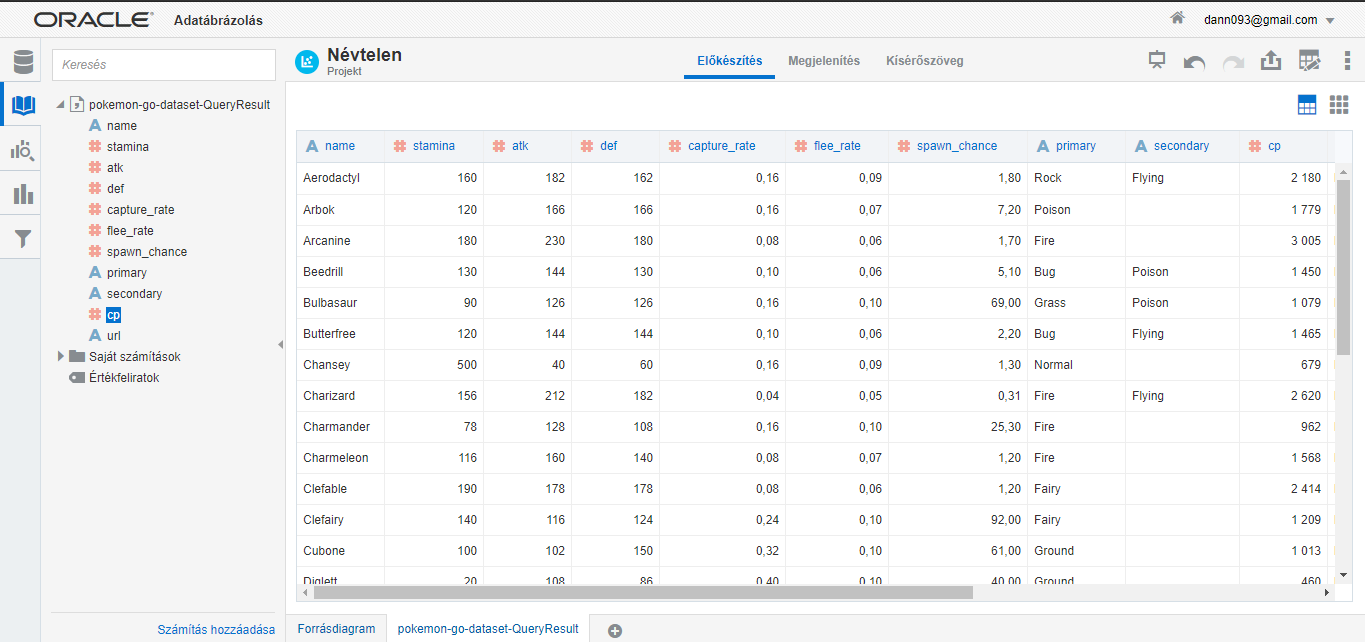
\includegraphics[width=1.0\linewidth]{dani_imgs/poke_data}
	\caption{Pokemon adathalmaz felépítése}
	\label{fig:pokedata}
\end{figure}

	\subsection{Egyedek összehasonlítása - Pontokból álló grafikon segítségével}
	Tegyük fel, hogy a célunk az egyedek kompetenciájának meghatározása bizonyos kritériumoknak megfelelően. A pont grafikon éppen alkalmas erre a célra. Az X tengelyhez hozzárendeljük az adott egyed védekező képességét, míg az Y tengelyhez az egyed támadó képességét. Ezáltal kapunk egy összefogó képet arról, hogy a lényeg képességek alapján hol helyezkednek el egymáshoz képest. Ezt a reprezentációt a \ref{fig:pokedata1}. ábra mutatja be.
	\begin{figure}[h!]
		\centering
		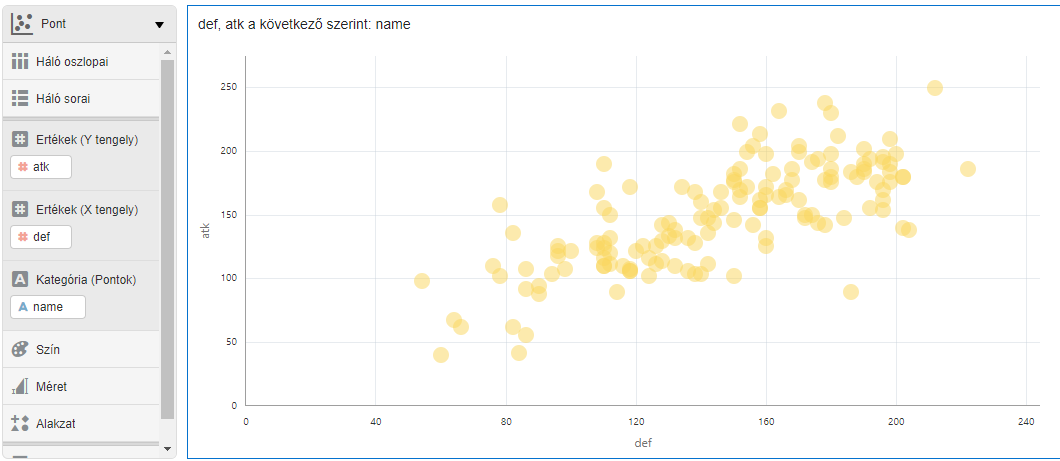
\includegraphics[width=0.85\linewidth]{dani_imgs/poke_data1}
		\caption{Egyed kompetenciák ábrázolása X-Y tengelyen}
		\label{fig:pokedata1}
	\end{figure}
	
	Azonban az egyszerű X-Y ponthalmaz grafikonnál jóval többre képes az eszköz, hiszen nem csak a térbeli pozíciója képes információt hordozni egy adott pontnak, hanem annak mérete, alakja és színe is. Ezt a bővített infografikus megjelenítést mutatja be a \ref{fig:pokedata2}. ábra. Itt már jobban a pontok mérete alapján eldönthető az egyed tényleges fejlődési potenciálja, illetve a fő típusa is egyből látszik. Ez a nézet például a játékban igen hasznos lehet, hiszen csapat építésnél könnyebben tudjunk megtalálni a számunkra értékesebb egyedet a sok közül.
	\begin{figure}[h!]
		\centering
		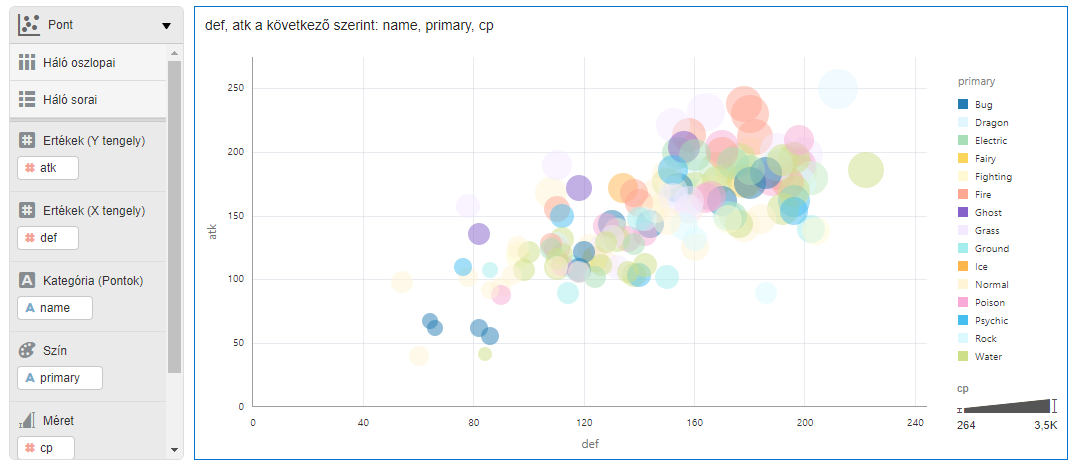
\includegraphics[width=0.85\linewidth]{dani_imgs/poke_data2}
		\caption{Egyed kompetenciák ábrázolása X-Y tengelyen bővített információtartalommal}
		\label{fig:pokedata2}
	\end{figure}

	Egyes megjelenítések igen sok adatot képesek vizualizálni, így könnyű elveszni bennük. A rendszer azonban igen segítőkész, ahogy a \ref{fig:pokedataexplain}. ábrán is látszik, minden megjelenítéshez tartozik egy informatív nézet, amely mutatja, hogy egyes mezők tartalma éppen milyen hatással van a megjelenítésre.	
	\begin{figure}[h!]
		\centering
		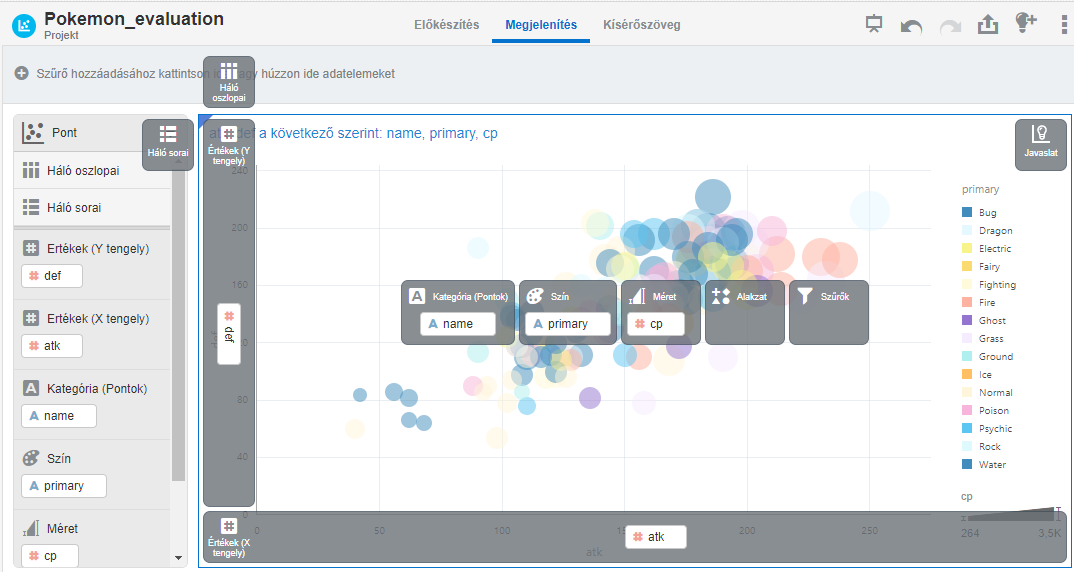
\includegraphics[width=0.7\linewidth]{dani_imgs/poke_data_explain}
		\caption{Beépített segítség, amely informatívan bemutatja az adat hozzárendeléseket a grafikonokon.}
		\label{fig:pokedataexplain}
	\end{figure}

	
	\subsection{Részletezés és szűrők}
	Nagyobb adatmennyiség esetén már nehezebben használható az ilyen jellegű megjelenítés. De tegyük fel, hogy tudjuk mit keresünk és szeretnénk például csak egy adott típust vizsgálni. Az eszköz támogatja különböző szűrők alkalmazását az adatokra, ezáltal ha például tudjuk, hogy minket csak a Ghost, Electic és Fire típusok érdekelnek, rászűrhetünk az adott tulajdonságra a \ref{fig:pokedatafilter}. ábrán látható módon. Az ábrán látszik, hogy hozzá lett adva a Water típus is a szűrőhöz, azonban annak a láthatósága ki-be kapcsolható. A későbbiekben kikapcsoltam, így a rendszer azt kiszürkítette, és abba a kategóriába tartozó adatok sem jelennek meg.
	\begin{figure}[h!]
		\centering
		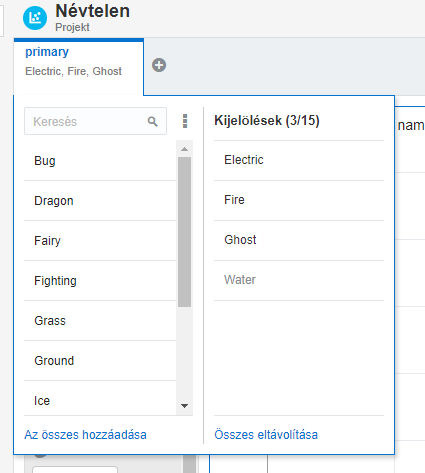
\includegraphics[width=0.5\linewidth]{dani_imgs/poke_data_filter}
		\caption{Szűrők beállítsa}
		\label{fig:pokedatafilter}
	\end{figure}
	A szűrő alkalmazás után, a megjelenített grafikon azonnal megváltozik, és csak a szűrt elemeket helyezi fel a \ref{fig:pokedatafilterresult}. ábrán látható módon. Az egyedekről bővebb információ nyerhető azokra rákattintva.
	\begin{figure}[h!]
		\centering
		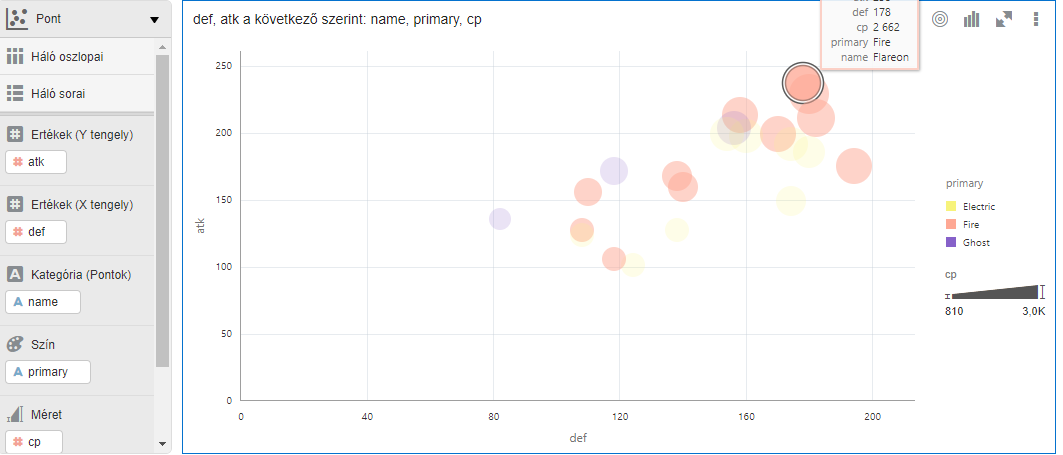
\includegraphics[width=0.85\linewidth]{dani_imgs/poke_data_filter_result}
		\caption{Egyed kompetenciák ábrázolása X-Y tengelyen, szűrők alkalmazásával}
		\label{fig:pokedatafilterresult}
	\end{figure}

	\subsection{Mutatós és informatív megjelenítés}
	Ebben az alfejezetben a címkefelhő megjelenítéssel foglalkozom, amely három érték alapján képes egy informatív kép előállítására. A címkefelhő lényegében a bemenetére adott címkéket helyezi el. Azonban ez tovább testre szabható, ha a színekhez attribútumot, és a betűmérethez pedig valamilyen metrikát rendelünk. Az azonos attribútummal rendelkező egyedek (jelen esetben azonos típusba tartozó pokemonok) azonos címmel kerülnek megjelenítésre, ezen felül pedig a magasabb cp-vel (combat power) rendelkezők egyedek pedig nagyobb betűmérettel rendelkeznek. Természetesen itt is alkalmazható az előző fejezetben alkalmazott szűrő, így készíthető az összes egyedet magába foglaló címkefelhő, mint az a \ref{fig:pokedatacime}. ábrán látható, de akár a típusok alapján is pár kattintással átrendezhető a címkefelhő, hogy csak a kívánt tulajdonságú egyedetek tartsa meg (lásd: \ref{fig:pokedatacimefiltered}. ábra)
	\begin{figure}
		\centering
		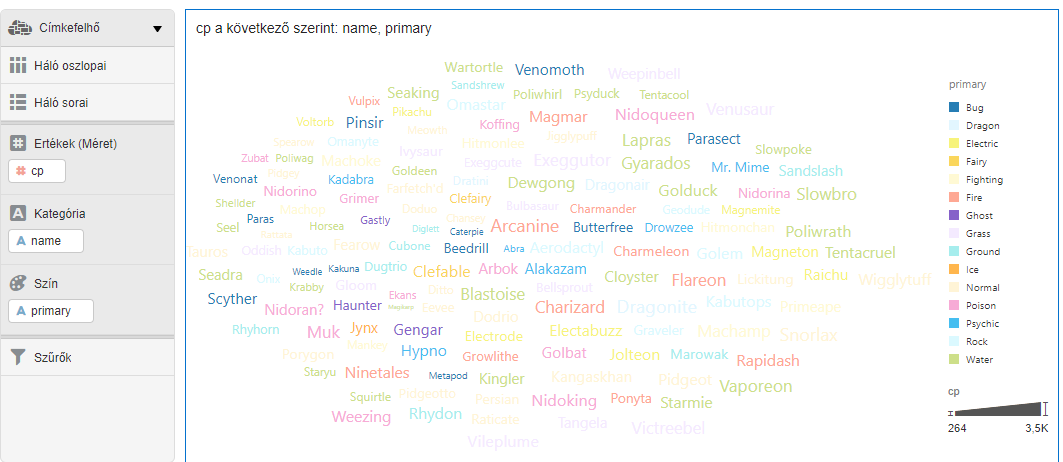
\includegraphics[width=0.7\linewidth]{dani_imgs/poke_data_cime}
		\caption{Címkefelhő az összes egyed használatával}
		\label{fig:pokedatacime}
	\end{figure}
	
	\begin{figure}
		\centering
		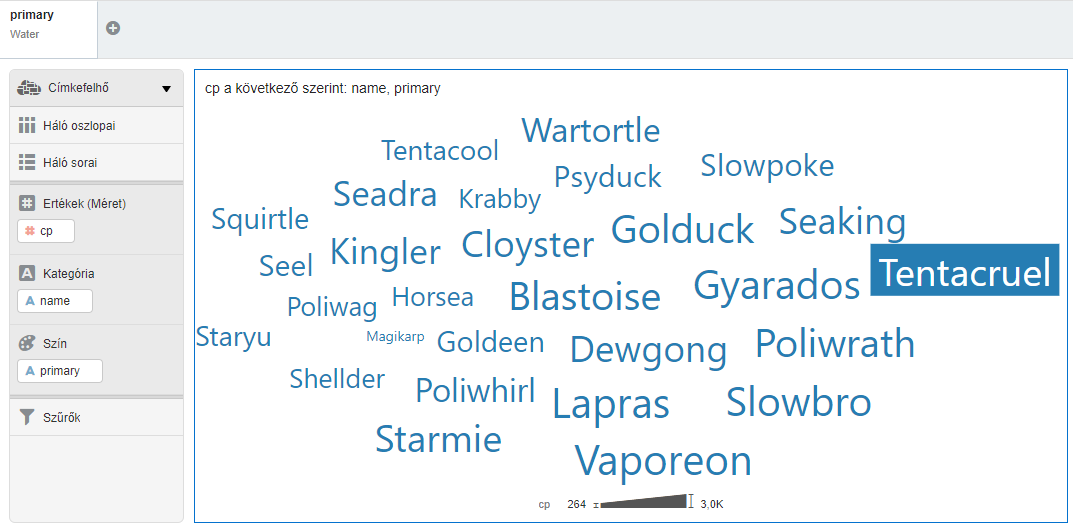
\includegraphics[width=0.7\linewidth]{dani_imgs/poke_data_cime_filtered}
		\caption{Címkefelhő attribútumra szűrve}
		\label{fig:pokedatacimefiltered}
	\end{figure}
	
	
	